\section{Completely Randomized Design}

We assume for the moment that the experimental units are homogeneous. We know how to compare two independent groups using the two-sample t-test. If we have more than two groups, this is not applicable anymore.


\subsection{One-Way Analysis of Variance}

On an abstract level we want to compare $g \geq 2$ treatments, having $N$ experimental units, that we assign randomly to the different treatment groups having $n_i$ observations each. This is what we call \textbf{completely randomized design}, it is the most elementary experimental design. If all the treatment groups have the same number of experimental units, we call the design \textbf{balanced}. Such random assignments can be done as follows:

\begin{lstlisting}
sample(treat.ord) ## Random Permutation of treat.ord
\end{lstlisting}

\subsubsection{Cell Means Model}

Let $y_{ij}$ be the observed response from the $j$-th experimental unit in treatment group $i$. In the \textbf{cells mean model} we allow each treatment group (cell) to have its own expected value. This means that $y_{ij}$ is the realised value of the random variable:
$$Y_{ij} \sim \mathcal N(\mu_i, \sigma^2), \; \text{ or } \; Y_{ij} = \mu_i + \epsilon_{ij}, \;\; \epsilon_{ij} \sim \mathcal N(0, \sigma^2)$$

As for the standard two-sample t-test, the variance is assumed to be equal for all groups. We say that $Y$ is the response and the treatment allocation is a categorical predictor. A categorical predictor is also called a factor. We sometimes distinguish between unordered (or nominal) and ordered (or ordinal) factors. We can rewrite the equation as:
$$\mu_i = \mu + \alpha_i$$

Where $\alpha_i$ is called the \textbf{treatment effect}. This will later help us to untangle the influence of multiple treatment factors on the response. Through this rewrite we have introduced an additional parameter, to remove it again we need a side constraint. Possible constraints could be:

\begin{itemize}
	\item weighted sum-to-zero: $\sum_{i=1}^{g} n_i \alpha_i = 0$
	\item sum-to-zero: $\sum_{i=0}^g a_i = 0$
	\item reference group: $\alpha_1 = 0$
\end{itemize}

For all of the choices it holds that $\mu$ determines some sort of "global level" of the data and $\alpha_i$ contains information about differences between the group means $\mu_i$ from that "global level". If we know $g-1$ of the $\alpha_i$, we automatically know the remaining $\alpha_i$, we also say that the treatment effect has $g-1$ \textbf{degrees of freedom} (df).

\begin{lstlisting}
## Options takes two args, the first for unordered 
## and the second for ordered factors.
## contr.poly        (weighted sum-to-zero) DEFAULT
## contr.sum         (sum-to-zero)
## contr.treatment (reference group)
options(contrasts = c("contr.sum", "contr.poly"))
\end{lstlisting}

\subsubsection{Parameter Estimation}

We estimate the parameters using the least squares criterion:
$$\hat \mu, \hat \alpha_i = \argmin{\mu, \alpha_i} \sum_{i=1}^g \sum_{j=1}^{n_i}(y_{ij} - \mu - \alpha_i)^2$$

Some notation:
\begin{align*}
	y_{i.} &= \sum_{j=1}^{n_i}y_{ij} 			  \qquad \qquad  \bar y_{i.} = \frac{1}{n_i}y_{i.}\\
	y_{..} &= \sum_{i=1}^g \sum_{j=1}^{n_i}y_{ij} \qquad \ \bar y_{i.} = \frac{1}{N} y_{..}
\end{align*}

As we can independently estimate the values of $\mu_i$, one can show that $\hat \mu_i = \bar y_{i.}$. From $\hat \alpha_i = \hat \mu_i - \hat \mu$ we can get all the other parameters needed (they still depend on the side constraint). \medskip

The estimate of the error variance is also called \textbf{mean squared error} $MS_E$:
$$\hat \sigma^2 = MS_E = \frac{1}{N - g} SS_E$$

Where $SS_E$ is the \textbf{error} or \textbf{residual sum of square}:
$$SS_E = \sum_{i=1}^g \sum_{j=1}^{n_i}(y_{ij} - \hat \mu_i)^2$$

We can fit the model as follows:
\begin{lstlisting}
fit <- aov(dresponse ~ dfactor, data = d)
## Go get the estimated coefficients
coef(fit) ## or dummy.coef(fit)
\end{lstlisting}

\subsubsection{Tests}

With the two-sample t-test, we could test whether two samples share the same mean. We will now extend this for $g > 2$. Saying that all groups share the same mean is equivalent to saying:
$$Y_{ij} = \mu + \epsilon_{ij}, \; \; \epsilon_{ij} \sim \mathcal N(0, \sigma^2)$$

This is the so-called \textbf{single mean model}, a special case of the cell means model. We have the global null hypothesis
$$H_0 : \mu_1 = ... = \mu_g$$

vs. the alternative hypothesis
$$H_A : \mu_k \neq \mu_l \text{ for at least one pair } k \neq l$$

The idea is to check whether the variation between the different treatment groups (the "signal") is  larger than the variation within the groups (the "noise"). We can decompose the total variation as follows:
$$\underbrace{\sum_{i=1}^g \sum_{j=1}^{n_i}(\bar y_{ij} - \bar y_{..})^2}_{SS_T} = \underbrace{\sum_{i=1}^g \sum_{j=1}^{n_i}(\bar y_{i.} - \bar y_{..})^2}_{SS_{Trt}} + \underbrace{\sum_{i=1}^g \sum_{j=1}^{n_i}(y_{ij} - \hat \mu_i)^2}_{SS_E} $$

This information can be summarized in a \textbf{ANOVA} table.
\begin{center}
	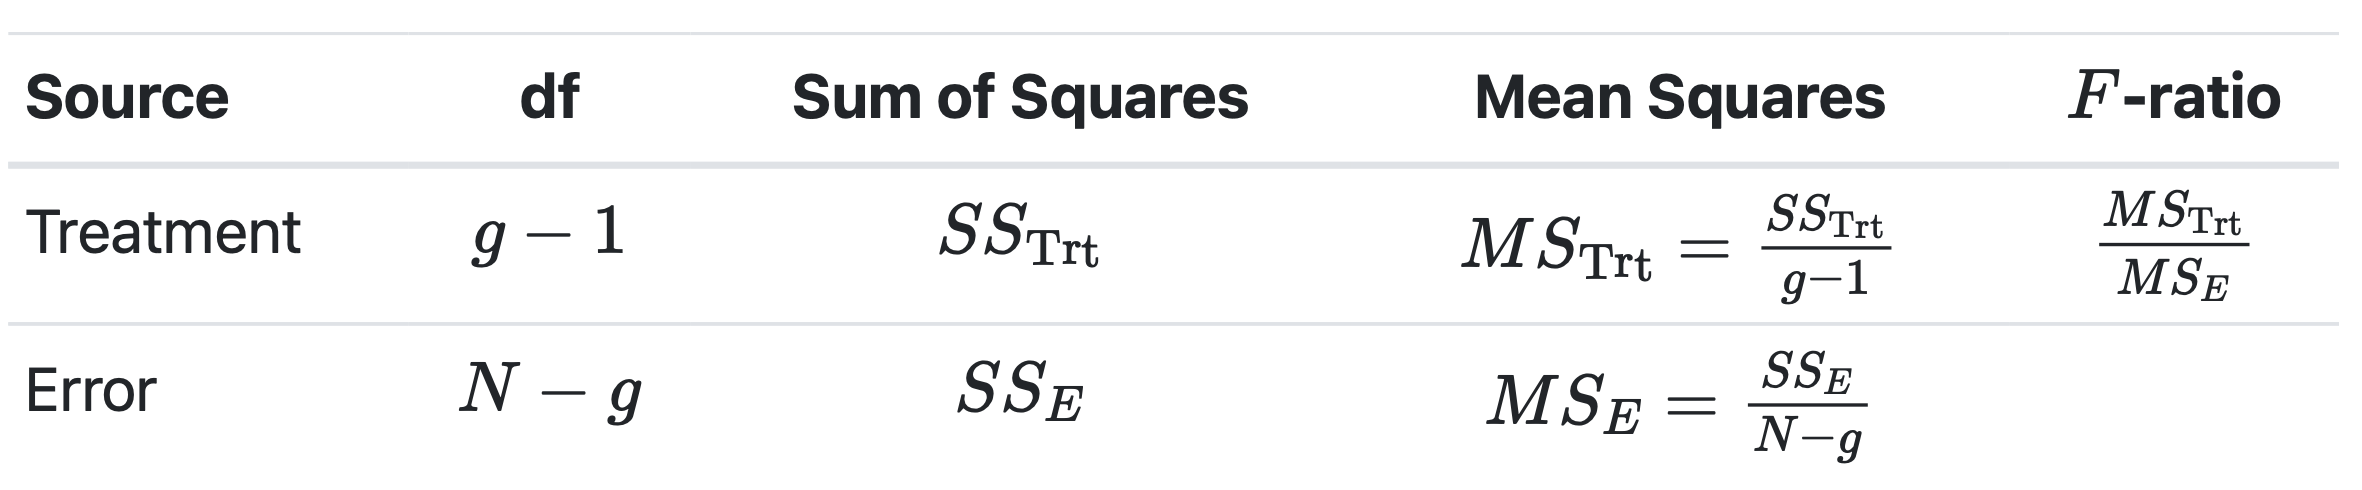
\includegraphics[width=\linewidth]{anova-table.png}
\end{center}

The $MS$ and $SS$ are normalized with the corresponding degrees of freedom. This is a so-called one-way ANOVA, because there is only one factor involved. If all groups share the same expected value, the treatment sum of squares is typically small. We introduce the so called $F$-ratio.
$$F\text{-ratio } = \frac{MS_{Trt}}{MS_E} \sim F_{g-1, N-g}$$

If the variation between groups is substantially larger than the variation within groups (higher $F$-ratio), we have evidence against $H_0$. The $F$-distribution looks as follows:
\begin{center}
	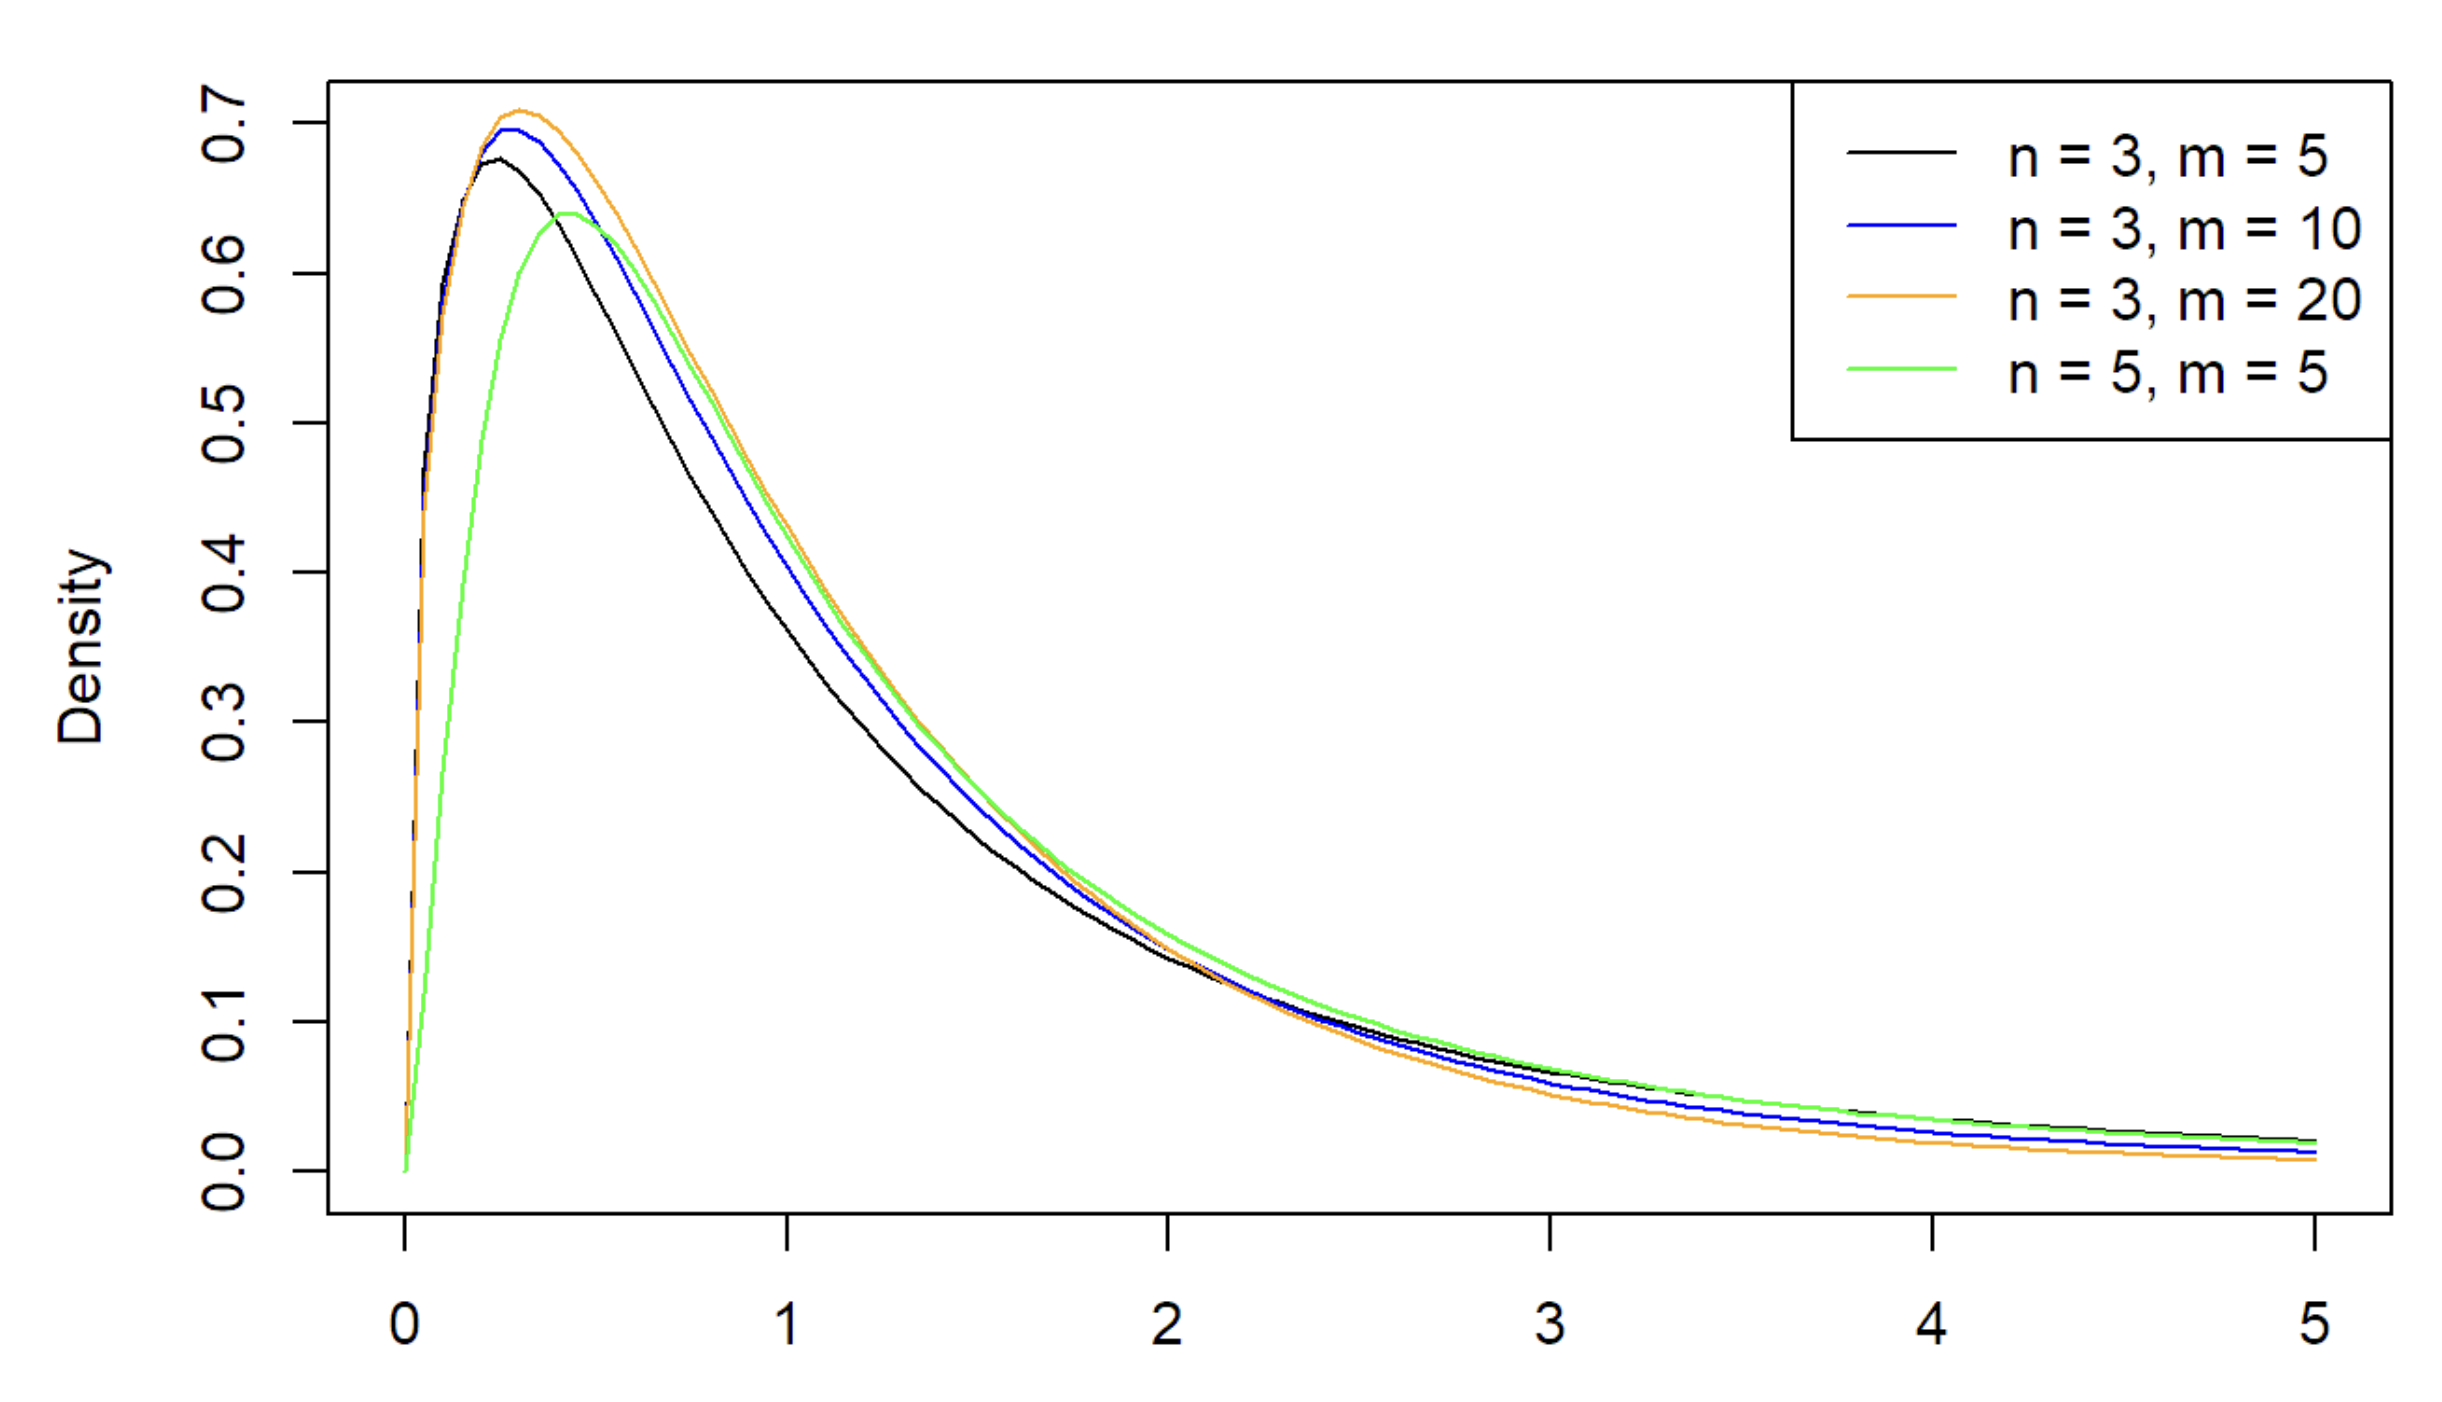
\includegraphics[width=\linewidth]{f-distribution.png}
\end{center}

As with any other statistical test, we reject $H_0$ if the observed value of the $F$-ratio, our test statistics, lies in an "extreme" region of the corresponding $F$-distribution:
$$F \text{-ratio} > F_{g-1, N-g, 1 - \alpha}$$

As this test is based on the $F$-ratio we call it an \textbf{$F$-test}. In R, we can use the following function to get the ANOVA table and the $p$-value of the $F$-test.
\begin{lstlisting}
summary(fit)
##             Df Sum Sq Mean Sq F value Pr(>F)
## group        2   3.77    1.883     4.85   0.016
## Residuals   27  10.49    0.389
\end{lstlisting}

To perform statistical inference for the individual $\alpha_i$'s we use:
\begin{lstlisting}
summary.lm(fit)   ## for the tests
confint(fit)      ## for the confidence intervals
\end{lstlisting}

\subsection{Checking Model Assumptions}

Statistical inference is only valid if all model assumptions are fulfilled. So far this means:
\begin{itemize}
	\item The errors are independent
	\item The errors are normally distributed
	\item The error variance is constant
	\item The errors have mean zero
\end{itemize}

We now introduce different plots to check these assumptions. This means that we use graphical tools to perform qualitative checks.

\subsubsection{QQ-Plot}

In a QQ-plot we plot the empirical quantiles of the residuals vs. the theoretical quantiles. The plot should show a more or less straight line if the normality assumption is correct.
\\[-20pt]
\begin{center}
	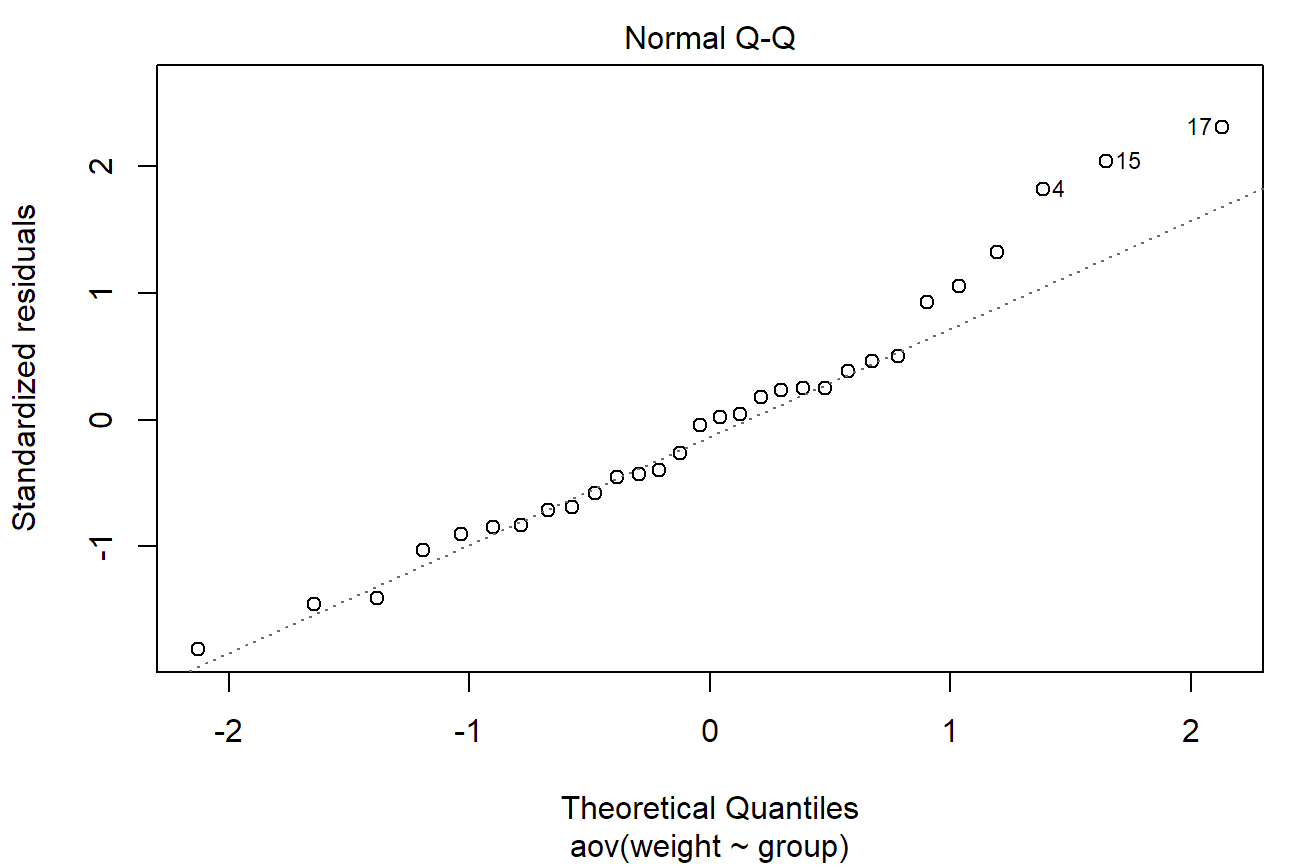
\includegraphics[width=\linewidth]{qq-plot.png}
\end{center}
\begin{lstlisting}
plot(fit, which = 2)
\end{lstlisting}

\subsubsection{Tukey-Anscombe Plot}

The Tukey-Anscombe plot (TA-plot) plots the residuals $r_{ij}$ vs. the fitted values $\hat \mu_i$ (estimated cell means). It allows us to check whether the residuals have constant variance.
\begin{center}
	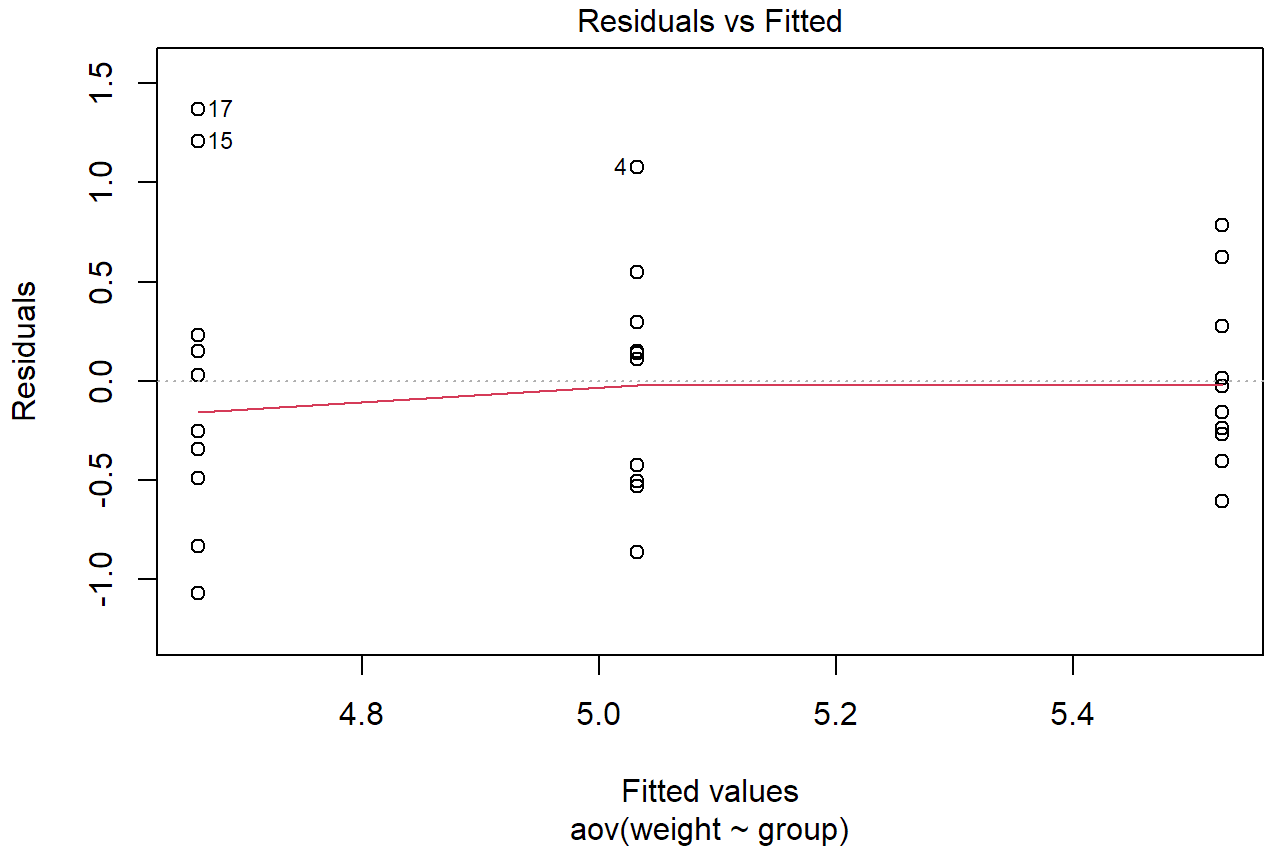
\includegraphics[width=\linewidth]{ta-plot.png}
\end{center}
\begin{lstlisting}
plot(fit, which = 1)
\end{lstlisting}

\subsubsection{Index Plot}

If the data has some serial structure, i.e. a certain time order, we typically want to check whether residuals close in time are more similar than residuals far apart. For this we use the index plot. For positively dependent residuals, we would see time periods where most residuals have the same sign, while for negatively dependent residuals, the residuals would “jump” too often from positive to negative compared to independent residuals. 
\begin{center}
	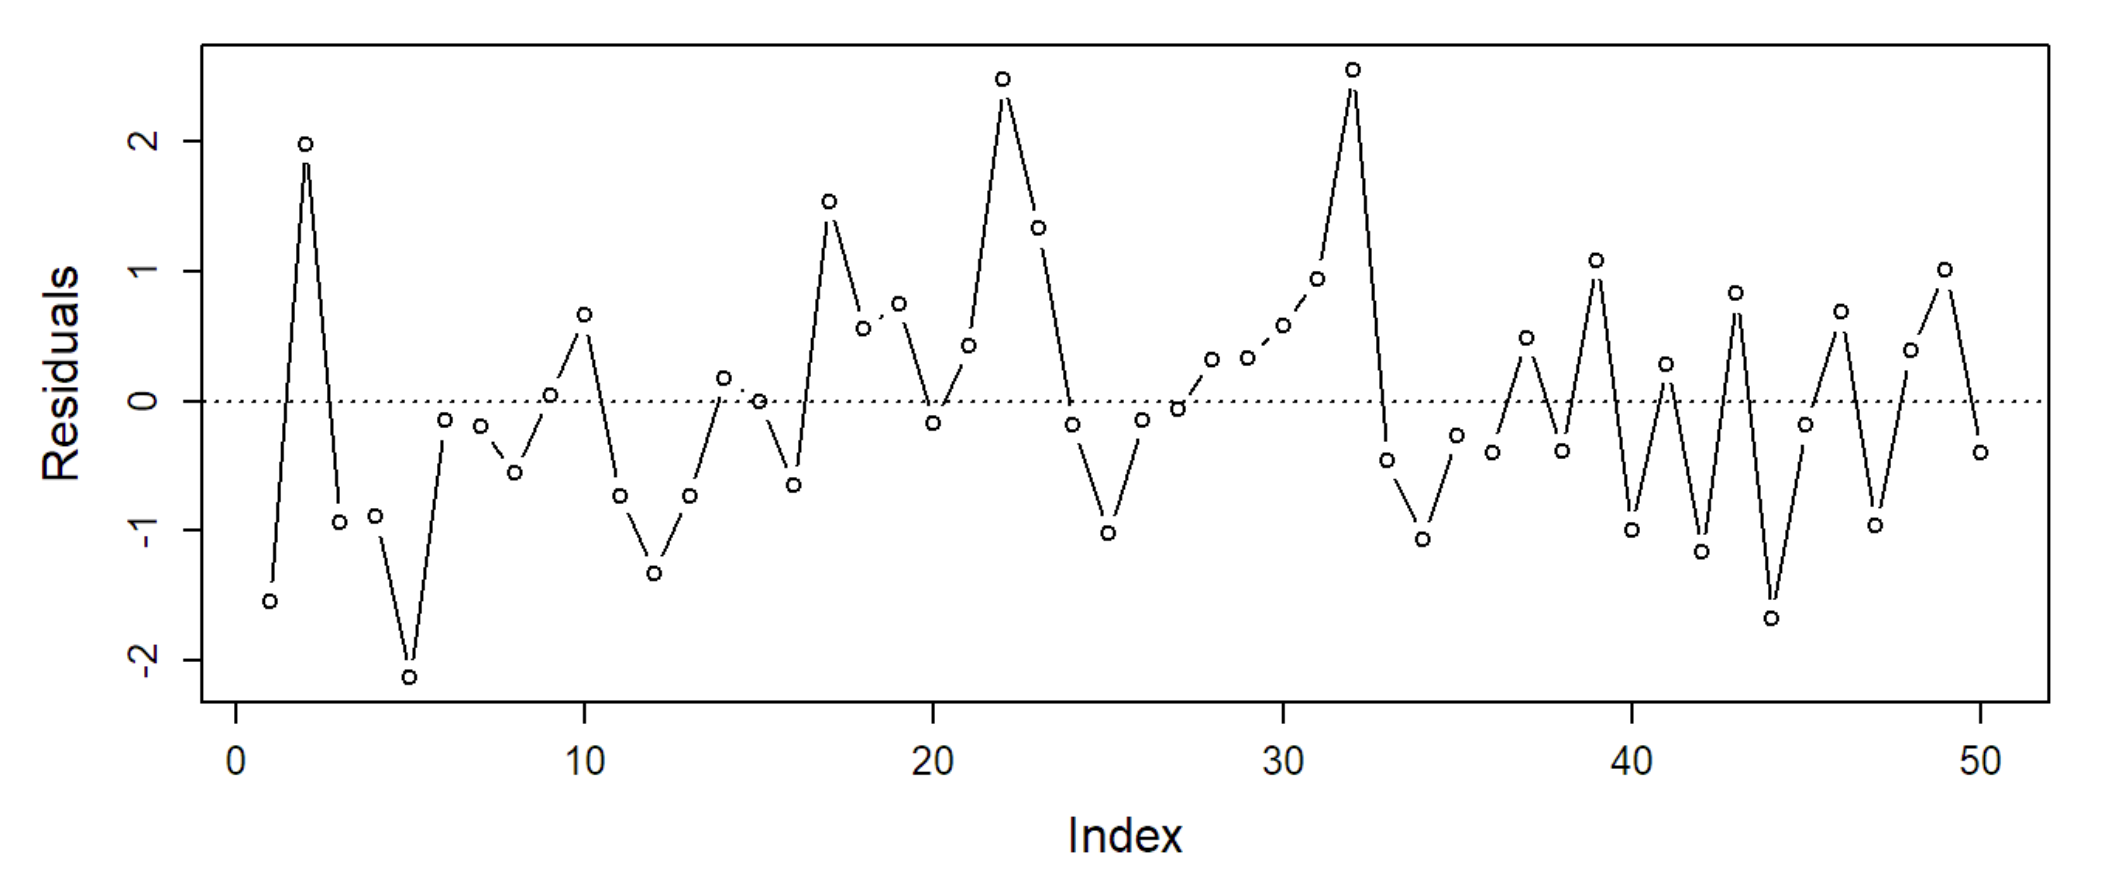
\includegraphics[width=\linewidth]{index-plot.png}
\end{center}


\subsection{Power / What Sample Size Do I Need?}

By construction, a statistical test controls the so-called type I error rate with the significance level $\alpha$. This means that the probability that we falsely reject $H_0$ is less than or equal to $\alpha$. Besides the type I error, there is also a type II error. It occurs if we fail to reject $H_0$ even though $H_A$ holds. The probability of a type II error is typically denoted by $\beta$. \medskip

The \textbf{power} of a statistical test is defined as \textit{P}(reject $H_0$ given that a certain setting under $H_A$ holds) = $1 - \beta$. Intuitively, it seems clear that the "further away" we choose the parameter setting from $H_0$ the larger will be the power, or the smaller will be the probability of a type II error.

\subsubsection{Calculating Power for a Certain Design}

Why should we be interested in such an abstract concept when planning an experiment? Power can be thought of as the probability of success, i.e. getting a significant result. The question of "what sample size do I need?" depends on the question of "what power do I want". The power depends on:
\begin{itemize}
	\item design of the experiment
	\item significance level
	\item parameter setting under the alternative
	\item sample size
\end{itemize}

We mainly use sample size and experimental design to maximize the power. Instead of doing the exact calculations, we rather choose an alternative way. We can always simulate a lot of data sets under $H_A$ that we believe in and check how often we are rejecting the corresponding $H_0$. The empirical rejection rate is then an estimate of the power. A nice side effect of doing a power analysis is that you actually do the whole data analysis on simulated data and you immediately see whether it works as intended. From a conceptual point of view, we can use such a simulation-based procedure for any design. However, the number of parameters grows rather quickly with increasing model complexity. \medskip

In that sense, the results of a power analysis are typically not very precise. However, they should still give us a rough idea about the required sample size in the sense of whether we need 6 or 60 observations per group.\medskip

In R we can calculate the power for simple designs like this:
\begin{lstlisting}
mu <- c(57, 63, rep(60, 3)) 
sigma2 <- 7 

## This will give us the estimated power
power.anova.test(groups = length(mu), n = 4, between.var = var(mu), within.var = sigma2)

## We can replace the argument n with power to get 
## and estimate for the needed sample size per group
power.anova.test(groups = length(mu), between.var = var(mu), within.var = sigma2, power = 0.8)
\end{lstlisting}
